\section{SOLID (8P)}
\subsection{Analyse SRP (3P)}
\task{jeweils eine Klasse als positives und negatives Beispiel für SRP; jeweils UML und Beschreibung der Aufgabe bzw. der Aufgaben und möglicher Lösungsweg des Negativ-Beispiels (inkl. UML)}
\subsubsection*{Positiv-Beispiel}
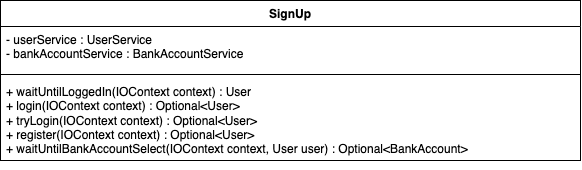
\includegraphics[width=\linewidth]{kapitel3_solid/SignUp.png}
Der BankAccountRestController ist eine Klasse, welche die CRUD-Endpunkte für die Bankkonten anbietet.
\subsubsection*{Negativ-Beispiel}
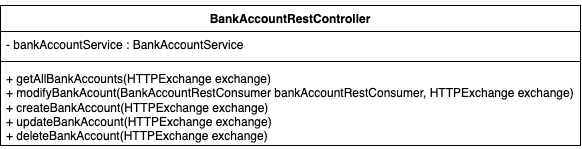
\includegraphics[width=\linewidth]{kapitel3_solid/BankAccountRestController.png}
Die SingUp-Klasse ist für das Anmelden und Registrieren eines Benutzers vor dem Programm dar. Dadurch das die Methoden waitUntilLoggedIn() sowie waitUntilBankAccountIsSelect() eher weniger mit dem Anmelden zu tun haben, müsste man diese in eine neue Klasse wie zum Beispiel WaitUntil extrahieren. 

\subsection{Analyse OCP (3P)}
\task{jeweils eine Klasse als positives und negatives Beispiel für OCP;  jeweils UML und Analyse mit Begründung, warum das OCP erfüllt/nicht erfüllt wurde – falls erfüllt: warum hier sinnvoll/welches Problem gab es? Falls nicht erfüllt: wie könnte man es lösen (inkl. UML)?}

\subsubsection*{Positiv-Beispiel}
Um auf der HTMLTag-Klasse aufzubauen wurde ein Interface daraus erstellt und Klassen wie HTMLTableRow oder HTMLTableCell erben von. HTMLTag die bestimmten Methoden. Somit wurde das OCP-Prinzip erfüllt. 
\newline\newline
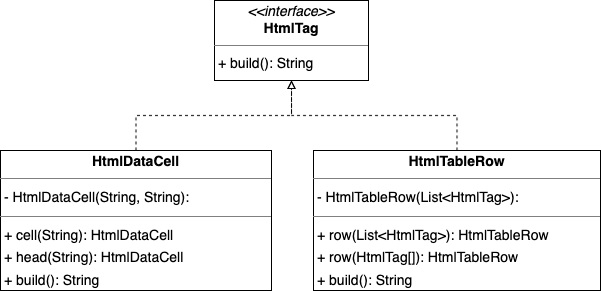
\includegraphics[width=\linewidth]{kapitel3_solid/positive_ocp.png}
\subsubsection*{Negativ-Beispiel}
\todo{Negativ Beispiel}
\subsection{Analyse [LSP/ISP/DIP] (2P)}
\task{jeweils eine Klasse als positives und negatives Beispiel für entweder LSP oder ISP oder DIP;  jeweils UML und Begründung, warum hier das Prinzip erfüllt/nicht erfüllt wird; beim Negativ-Beispiel UML einer möglichen Lösung hinzufügen}
\task{Anm.: es darf nur ein Prinzip ausgewählt werden; es darf NICHT z.B. ein positives Beispiel für LSP und ein negatives Beispiel für ISP genommen werden}

\subsubsection*{Positiv-Beispiel}
\todo{Positiv Beispiel}
\subsubsection*{Negativ-Beispiel}
\todo{Negativ Beispiel}